\documentclass[coguia]{tesis-usach}
% Opciones: coguia, propuesta
\usepackage{amsmath}
\usepackage{changepage}
\begin{document}
\baselineskip 23pt
\frontmatter								% Utiliza numeración romana

% ### Cubierta de la tesis ###
\thispagestyle{empty}
\facultad{Ciencia}
\departamento{Matemática y Ciencia de la \\Computación}
\grado{Analista en Computaci\'on Cient\'ifica}

\titulo{Un módulo para una herramienta computacional que detecta el estatus de un sistema de atención, basado en Teoría de Colas y el método de Monte Carlo}

\autor{Benjamín Nicolás Klerman Muñoz\\Fabián Venegas Bustamante}
\email{benjamin.klerman@usach.cl\\fabian.venegas@usach.cl}
\run{12.345.678-9}		% S\'olo necesario en propuesta
\telefono{22222222}		% S\'olo necesario en propuesta
\annoingreso{Año}

\fecha{Viernes}{28}{Enero}{2022}

\profesorguia{Mladen Nadinic Cruz}
%\profesorcoguia{Profesor(a) Co-Gu\'ia}

\ciudad{Santiago}
\pais{Chile}

\makecubierta


% ### Páginas preliminares de la tesis ###
\pagestyle{fancy}
\renewcommand{\headrulewidth}{0pt}		% Hace que no aparezca la línea horizontal superior al principio de estas páginas
\newcommand{\p}[1]{\left( #1 \right)}
\newcommand{\pc}[1]{\left[ #1 \right]}
\newcommand{\pb}[1]{\left\lbrace #1 \right\rbrace}
\newcommand{\pl}[1]{\left| #1 \right|}

\fancyhead[L]{}
\fancyhead[C]{}
\fancyhead[R]{}

{\setstretch{1.0}						% Interlineado en las páginas preliminares
\makecopyright							% Si es propuesta no se mostrará

% ### Resumen de la tesis
\setcounter{page}{0} 
\include{preliminares/abstract}

% ### Dedicatoria y agredecimientos de la tesis ###
\input{preliminares/dedicatoria}		% En caso de no querer agregarlos, comente esta línea
\input{preliminares/agradecimiento}

% ### Índices ###
\tableofcontents							%% Tabla de contenido

\listoftables							%% Indice de tablas
\listoffigures							%% Indice de figuras
\listofalgorithms						%% Indice de algoritmos (Optativo: En caso de poseer algoritmos)
\AtBeginEnvironment{algorithmic}{\setstretch{1.5}} % Interlineado de los algoritmos
} % end \setstretch{1.0}

% ### Cuerpo de la tesis ###
\mainmatter								% Reinicia el contador de páginas para partir de 1 y usando números arábicos.

% ### Capítulos de la tesis ###
\chapter{Introducci\'on}
\label{cap:introduccion}

\section{Antecedentes y motivaci\'on}
\label{intro:motivacion}
\begin{comment}
En 1981 el Sr. Marcelo Pardo Brown es contratado por la Universidad para crear el Departamento de Ingeniería Informática y la carrera de Ingeniería Civil en Informática. Oficialmente, el Departamento fue creado mediante el decreto 286 del 7 de mayo de 1982 y su primer director fue el Sr. Pardo. Ese mismo año, el Departamento asume la tutela de la carrera de Ingeniería de Ejecución en Computación e Informática \citep{Codishetal2000}.
\end{comment}


\section{Descripci\'on del problema}
\label{intro:problema}
\begin{comment}
La carrera de Ingeniería Civil en Informática se crearía oficialmente por Resolución 2324 de 1983.  Los primeros Ingenieros Civiles en Informática de la USACH comenzaron a titularse en el año 1987.

La creación del Departamento permitió entre otras cosas la implementación de un plan de contratación de profesores Jornada Completa y la elaboración de un plan de equipamiento computacional dedicado a las tareas académicas del Departamento. Hasta 1983, los alumnos realizaban sus tareas computacionales usando exclusivamente los recursos Computacionales de SECOM, que en ese entonces consistían principalmente en un computador IBM 370/145 con 256 Kilobytes de memoria. A mediados de los 80, el Departamento adquirió un computador VAX 730 que tenía 2 Megabytes de memoria RAM con el sistema operativo VMS. Además, se habilitó un primer centro de operaciones computacionales y las salas de terminales para uso exclusivo de los alumnos del Departamento.
\end{comment}

\section{Soluci\'on propuesta}
\label{intro:solucion}
\begin{comment}
Físicamente, el Departamento permaneció en las dependencias del Departamento de Ingeniería Industrial hasta 1988, cuando fue trasladado para ocupar lo que fuera el Pabellón de Forja de la Escuela de Artes y Oficios, edificio que es monumento histórico.

Las nuevas dependencias incluían seis salas de laboratorio para docencia, tres laboratorios de investigación para uso de memoristas, cuatro salas de clases, una biblioteca especializada, un centro de operaciones más amplio y apto para las nuevas necesidades tecnológicas del Departamento, oficinas para profesores, administrativos y secretarias docentes para cada carrera. También tuvo baños para uso exclusivo de los miembros del Departamento.

Sin duda este fue el comienzo de una nueva etapa en la vida del Departamento. Su imagen al interior de la Facultad y de la Universidad creció y se potenció con la participación de algunos académicos en proyectos institucionales, como la Dirección de SEGIC y la instalación de una red de fibra óptica en todo el campus universitario.
\end{comment}



\section{Objetivos y alcance del proyecto}
\label{intro:objetivos}

\subsection{Objetivo general}
\noindent Implementar un módulo de una herramienta computacional, utilizando la Teoría de Colas y el método de Monte Carlo para conocer el estatus de un sistema de atención.
% enfocar en MC, dejar TC para la parte metodológica de cómo se usará MC

\subsection{Objetivos espec\'ificos}
\begin{enumerate}
	\item Describir la metodología de desarrollo de la herramienta computacional.
	\item Analizar aplicaciones de la Teoría de Colas y Monte Carlo.
	\item Simular, mediante Monte Carlo, el comportamiento de las filas de espera en el comercio.
	\item Implementar módulo de prueba para la herramienta computacional

\end{enumerate}

\subsection{Alcances}
\begin{comment}
En el año 1993 se creó mediante Resolución 1662 la Prosecución de Estudios conducentes al título de Ingeniero Civil Informático, modalidad vespertina. Este programa de formación está dirigido a profesionales titulados de carreras de Ingeniería de Ejecución del área.

Adicionalmente, un proyecto de equipamiento mayor permitió la compra de un Super-Computador Silicon Graphics para procesamiento paralelo, único en ese momento en el país. Aparece entonces la necesidad de crear tres laboratorios de investigación en las áreas de Procesamiento Paralelo y Optimización, Sistemas Colaborativos y Robótica. La creación de estos laboratorios y la creciente implicación de alumnos como ayudantes de investigación, permitieron abordar proyectos señeros de Asistencia Técnica, como la elaboración de un manual de entrenamiento para el avión Pillán de la Fuerza Aérea de Chile, basado en tecnologías de realidad virtual.
\end{comment}


\section{Metodolog\'ia y herramientas utilizadas}
\label{intro:metodologia}

\subsection{Metodolog\'ia}
\begin{comment}
Se creó el primer programa de titulación especial para ex-alumnos y la carrera de Ingeniería de Ejecución en Computación e Informática modalidad vespertina.
\end{comment}


\subsection{Herramientas de desarrollo}
\begin{comment}
El Departamento comenzó a potenciar sus actividades de investigación mediante la creación del Magíster en Ingeniería Informática (Resolución 386 de 1994), y la implantación de un plan de perfeccionamiento para los académicos conducente a la obtención del grado de Doctor. El plan además consideraba la contratación de nuevos académicos con dicho grado. Es así, como a finales de los 90, el Departamento contaba con nueve doctores jornada completa y otros dos en perfeccionamiento.
\end{comment}


\section{Organizaci\'on del documento}
\label{intro:organizacion}
\begin{comment}
Contar con este grupo de académicos con grado de doctor permitió alcanzar una masa crítica que, junto con los resultados exitosos del Magíster en Ingeniería Informática, motivó al Departamento a trabajar en la elaboración del Programa de Doctorado en Ciencias de la Ingeniería mención Informática. Este programa fue creado por Resolución 6104 del 2000. Ese mismo año el Departamento organizó con éxito las Jornadas Chilenas de Computación, punto de reunión de los académicos nacionales y de los alumnos de Informática del país y que contó además con la participación de destacados investigadores de orden mundial.
\end{comment}

\chapter{Cuerpo de la tesis}
\label{cap:cuerpo}
%%%%%%%%%%%%%%%%%%%%%%%%%%%%%%%%%%%%% MARCO Teórico
\section{Primera parte: Marco Teórico} % check 10/24
\label{sec:primera}

\noindent En esta sección se expondrán los conceptos centrales que se abordarán y utilizarán a lo largo del trabajo de tesis. Las primeras dos subsecciones tratan específicamente de Simulaciones de Monte Carlo y Teoría de Colas, pasando a explicar en una tercera sub sección, la integración de ambos conceptos y posterior a eso, hablar sobre usos que le ha dado a estos temas en el mundo real, visto desde el punto de vista de aplicaciónes y herramientas de software.

\subsection{Simulación de Monte Carlo} %check 10/24

\noindent A continuación, se presenta el concepto de Simulación de Monte Carlo. Se inicia por explicar sus origenes historicos, para luego proceder a hablar sobre en qué consiste este, detalles o alcances a tener cuenta sobre el mismo, los fundamentos que le dan sustento matemático, terminando con ejemplos a fin de entender más a cabalidad el funcionamiento y usos que se le pueden dar, así como dar cuenta de las variadas áreas que se pueden abordar con Simulaciones de Monte Carlo.

\subsubsection{Historia} % check 10/24

\noindent El concepto de \textit{método de Monte Carlo} data sus inicios a la segunda guerra mundial buscando simular el comportamiento de neutrones de materias fisionables \citep{haro2021}. La ideación de este se adjudica a los científicos Stanislaw  Ulam y John von Neumann, quienes a mediados de la decada de 1940s, en el marco del desarrollo de proyectos de armas nucleares, propusieron dicha teoría, que posteriormente fue puesta a prueba dentro de las simulaciones del proyecto Manhattan. Tratándose de un proyecto delicado y altamente secreto, Nicholas Metropolis, colega de Ulam y von Neumann, sugirió Monte Carlo como nombre clave, debido a la a afición de von Neumann por la aleatoriedad de las cosas y los juegos de azar \citep{metropolis1987}. Lo que proponían Ulam y von Neumann era un proceso de estudio sobre una secuencia numérica (o de estados representados numéricamente) cuyos valores derivan de probabilidades aleatorias.
\newline \newline
Hacia la segunda mitad del siglo XX, se encuentran muchas publicaciones de diversas áreas (matemáticas, física, química molecular, etc.) basadas en la aplicación de Monte Carlo en distintas situaciones, sin embargo estas carecían de fundamentos centrales o simplemente no incurrian en la discusión sobre estimadores o algoritmos que probaron ser fundamentales en el desarrollo de este método. Pero fue a finales del mismo siglo que aparecieron autores que propusieron metodologias ligadas a las variaciones en el tamaño de la población, poniendo sobre la mesa nuevamente temas elementales sobre la teoría detras de Monte Carlo, dando paso a otros desarrollos en el área empezando el nuevo siglo \citep{delmoral1997,delmoral1998,crisan1998,delmoral2001}.
%Del Moral, Pierre (1996). "Non Linear Filtering: Interacting Particle Solution" (PDF). Markov Processes and Related Fields. 2 (4): 555–580.
%Del Moral, Pierre (1998). "Measure Valued Processes and Interacting Particle Systems. Application to Non Linear Filtering Problems". Annals of Applied Probability (Publications du Laboratoire de Statistique et Probabilités, 96-15 (1996) ed.). 8 (2): 438–495. CiteSeerX 10.1.1.55.5257. doi:10.1214/aoap/1028903535
%Crisan, Dan; Gaines, Jessica; Lyons, Terry (1998). "Convergence of a branching particle method to the solution of the Zakai". SIAM Journal on Applied Mathematics. 58 (5): 1568–1590. doi:10.1137/s0036139996307371. S2CID 39982562
%Del Moral, Pierre; Guionnet, Alice (2001). "On the stability of interacting processes with applications to filtering and genetic algorithms". Annales de l'Institut Henri Poincaré. 37 (2): 155–194. Bibcode:2001AnIHP..37..155D. doi:10.1016/s0246-0203(00)01064-5

\subsubsection{Concepto general} % check 10/24
\noindent Si bien existe una gran cantidad de definiciones para las simulaciones o métodos de Monte Carlo, no existe un real consenso que englobe el concepto de manera general. Sin embargo, Ulam, en su autobiografía, explicaba el cálculo de Monte Carlo con el siguiente ejemplo: 

\begin{adjustwidth}{1.27cm}{}
 Suponga que desea estimar la probabilidad de ganar una partida de Solitario, asumiendo que la baraja de cartas está perfectamente revuelta antes de comenzar. Una vez  que se hayan escogido las estrategias para colocar una pila de cartas sobre otras, el  problema es derechamente la teoría de probabilidad, pero una muy tediosa. No sería  complicado programar una computadora para \textit{randomizar} listas que representen  las 52 cartas de una baraja, preparar listas que representen las distintas pilas,  y luego simular la partida de juego hasta su final. La observación de muchas  repeticiones llevaría a un estimado de Monte Carlo acerca de una posibilidad de éxito.  Este método, de hecho, sería la forma más fácil de realizar cualquier estimado.  Podemos considerar el juego de la computadora como una fiel simulación del real  proceso aleatorio de revolver y ordenar las cartas \citep{kalos2008}.
\end{adjustwidth}
~
\newline
De lo anterior, entonces, se puede concluir que Monte Carlo consiste en simular una situación o fenómeno de la vida real, a partir de parámetros o valores establecidos, repitiendo de manera aleatoria el ensayo una cantidad de veces lo suficientemente grande como para que sus resultados sean verosímilies, así como para tener en cuenta casi cualquier posibilidad que pueda ocurrir dentro del fenómeno en estudio.
% citar?

\subsubsection{Detalles y apreciaciones} % check 10/24

\noindent Respecto a este tema, Sawilowsky plantea la diferencia entre los conceptos Simulación, Monte Carlo y Simulación de Monte Carlo \cite{sawilowsky2003}. En primer lugar, Simulación es elaborar un modelo abstracto de una situación real para poder comprender el impacto de modificaciones y el efecto de agregar diversas variaciones \citep{negoita1987}; en el caso del juego de solitario, una simulación de este podría ser una transcripción directa del proceso \citeyear{sawilowsky2003}. Y por otro lado, Monte Carlo, se entiende como un método para obtener un valor esperado a partir de la generación de grandes cantidades de valores pseudo aleatorios de manera uniforme (en el ejemplo del juego de solitario, Monte Carlo entrega una solución probabilistica para sucesos o problemáticas no probabilistas). De esta forma, se puede entender una Simulación de Monte Carlo como la generación pseudo aleatoria de valores aplicado en un modelo basado en una situación del mundo real. La distinción es bastante sutil, y muchas veces, difícil de distinguir. Sin embargo, la distinción de estos puntos, adquiere relevancia a la hora de plantear una buena formulación de una Simulación de Monte Carlo.
\newline \newline
\cite{sawilowsky2003} también postula que una Simulación de Monte Carlo de alta calidad debe incluir algunos factores imprescindibles para una correcta y útil simulación. Factores como:
\begin{itemize}
    \item La generación de números pseudo aleatorios se debe dar cada cierto periodo de tiempo establecido.
    \item La generación de números pseudo aleatorios entrega valores que aprueban pruebas de aleatoriedad.
    \item La cantidad de repeticiónes del experimento debe ser lo suficientemente grande para asegurar la precisión de los resultados.
    \item Se utiliza una técina de muestreo apropiada.
    \item El algoritmo es válido para el proposito que se le pretende dar.
    \item El estudio simula el fenómeno en cuestión.
\end{itemize}

\subsubsection{Fundamentos} %%% check 10/24

\noindent A continuación en esta sección, se verán brevemente algunos conceptos y teoremas que dan fundamento matemático a las simulaciones de Monte Carlo, como la Ley de Grandes Números, el Teorema fundamental de Monte Carlo y otros teoremas matemáticos afines de interés.

\begin{itemize}
    \item \textit{Ley de Grandes Números:}
    \newline
    Dentro de la idea de Monte Carlo de realizar varios experimientos para obtener una precisión más contundente y que da sustento matemático al método, se desprende la Ley de Grande Números, la cual propone que el promedio de los resultados de la repetición de alguna prueba se acerca al valor esperado de esta a mayor cantidad de repeticiones. Visto desde un punto de vista estadístico, el promedio de \textit{N} variables aleatorias iid $X_i , \Bar{X}_{N} = S_N / N$ converge a E[$X$] cuando \textit{N} es mayor, es decir,

    \begin{equation}
        \text{P} \bigg( \lim_{N \rightarrow \infty} \Bar{X}_{N} = E[X] \bigg) = 1
    \end{equation}

    De esta forma, se entiende que la esperanza de una variable aleatoria converge al promedio a medida que la muestra es de mayor tamaño, al realizar muestreos repetitivos \citep{dekking2005}.
    
    \item \textit{Desigualdad de Markov:}
    \newline
    Supongamos una variable aleatoria $X$ que solo toma valores no negativos, y sea $f$ su función de densidad de probablididad o pdf (como se denomina comúnmente). Entonces, para cualquier $x$ > 0,
    %%%%%%%%%%%%%%%%%% arreglar salto de linea
    \begin{align}
        \text{E}[X] = \int_{0}^{x} dt ~ t ~ f(t) + \int_{x}^{\infty} dt ~ t ~ &f(t) \geq \int_{x}^{\infty} dt ~ t ~ f(t) \newline \geq \int_{x}^{\infty} dt ~ x ~ f(t) = x \text{P} (X \geq x)\\
        &\Rightarrow \text{P}(X \geq x) \leq \dfrac{\text{E[X]}}{x}.
    \end{align}
    
    \citep{cohen2015}.
    
    \item \textit{Desigualdad de Chebyshev:}
    \newline
    Bajo el supuesto de que $\mu$ es la esperanza de $X$ y $\sigma^2$ es su varianza, entonces al aplicar la desigualdad de Markov sobre la variable aleatoria $D^2 = (X - \mu)^2$ (cuya esperanza también es $\sigma^2$), entrega como resultado que $\text{P}(D^2 \geq x^2) \leq \frac{\sigma^2}{x^2}$. Entonces,
    
    \begin{equation}
        \text{P}(\mid X - \mu \mid \geq x) \leq \dfrac{\sigma^2}{x^2}.
    \end{equation}
    
    \citep{dekking2005}
    
    \item \textit{Cálculo Monte Carlo:}
    \newline
    Consideremos una variable aleatoria $G_N$ como el promedio de una función $g(X_i)$ de variables iid,
    
    \begin{equation}
        G_N = \dfrac{1}{N} \sum_{i = 1}^{N} g(X_i)
    \end{equation}
    
    cuya esperanza y varianza son respectivamente
    
    \begin{equation}
        \text{E}[G_N] = \text{E}[g(X)], ~~~~ var(G_N) = \dfrac{var(g(X))}{N}.
    \end{equation}
    
    \citep{kalos2008}
    
    Al promedio $G_N$ se le llama \textit{estimador} de $\text{E}[g(X)]$, ya que su esperanza vale
    
    \begin{equation}
        \text{E}[G_N] = \text{E}[g(X)] = \int_{-\infty}^{\infty} dx ~ g(x) f(x)
    \end{equation}
    
    donde $X_i \sim f$.
    \newline \newline
    Dicho de otra forma, la integral en (2.7) se puede evaluar generando un conjunto de $N$ variables aleatorias $X_i$ según $f(x)$ y hayando $g(x)$ para cada una. La media aritmética de los $g(x)$ generados (2.5) entrega el valor de la integral (2.7). Ahora, también es cierto que la varianza del estimador disminuye al crecer $N$.
    \newline \newline
    Aplicando la desigualdad de Chebyshev (2.4) sobre la variable aleatoria $G_N$ con $\sigma^2 = \text{var}(G_N), x^2 = \frac{\sigma^2}{\delta}$ y $\delta > 0$ se obtiene
    
    \begin{equation}
        \text{P}\Bigg( \mid G_N - E[G_N] \mid \geq \bigg[ \dfrac{\text{var}(G_N)}{\delta} \bigg] ^{\frac{1}{2}} \Bigg) \leq \delta
    \end{equation}
    
    o utilizando (2.6)
    
    \begin{equation}
        \text{P}\Bigg( \mid G_N - E[g(X)] \mid \geq \bigg[ \dfrac{\text{var}(g(X))}{N \delta} \bigg] ^{\frac{1}{2}} \Bigg) \leq \delta
    \end{equation}
    
    Entonces, al generar una muestra lo suficienctemente grande $(N > \frac{1}{\delta})$ la probablididad de que el estimador se aleje del valor esperado de $g(X)$ puede ser tan pequeña como se requiera.
    
    \item \textit{Teorema central de límite:}
    \newline
    Para seguir profundizando, si la variable aleatoria $G_N$ toma valores $g_N$ y definimos
    
    \begin{equation}
        t_N = g_N - \dfrac{\text{E[g(X)]}}{\sqrt{\text{var}(G_N)}} = \dfrac{g_N - \text{E[g(X)]}}{\sqrt{\text{var}(g(X))} / \sqrt{N}}
    \end{equation}
    
    El teorema central de límite \citep{fischer2010}, abocado al contexto de Monte Carlo, indica que
    
    \begin{equation}
        \lim_{N \rightarrow \infty} \text{P}(a < t_N < b) = \int_{a}^{b} dt \dfrac{\text{e}^{-\frac{1}{2}t^2}}{\sqrt{2\pi}}
    \end{equation}
    
    Es decir que, cuando $N$ es muy grande, los valores de $G_N$ siguen una distribución normal de media $\mu = \text{E}[g(X)]$ y varianza $\frac{\sigma^2}{N}$ con $\sigma^2 = \text{var}(g(X))$. Con esto, se puede realizar el siguiente cambio de variable:
    
    \begin{equation}
        t_N = \dfrac{g_N - \mu}{\sigma / \sqrt{N}}, ~~~~ dt_N = \dfrac{dg_N}{\sigma / \sqrt{N}}
    \end{equation}
    
    Entonces, a partir de (2.11), en el límite de $N$ suficientemente grande, $G_N$ distribuye de la siguiente forma:
    
    \begin{equation}
        f_{G_{N}} (g_{N}) \rightarrow \dfrac{1}{\sqrt{2\pi} (\sigma / \sqrt{N})} \text{exp} \Bigg\{-\dfrac{1}{2} \bigg( \dfrac{g_N - \mu}{\sigma / \sqrt{N}} \bigg)^2 \Bigg\}, ~~~~ N > 1
    \end{equation}
    
    lo que se cumple para la distribución de una $f(x)$ cualquiera.
    %% fuente: Métodos Monte Carlo, Jose Ignacio Illana, 2013
    
    \item \textit{Método de la transformada inversa \citep{gonzalez2010}:}
    \newline
    Una vez vistos los elementos conceptuales que sirven de fundamento para el método y las simulaciones de Monte Carlo, resta puntualizar como se obtienen valores aleatorios. Como se mencionó anteriormente en esta sección, Monte Carlo contempla valores aleatorios generados uniformemente, sin embargo, en el mundo real abundan los fenómenos que siguen (o se traducen como) una distribución de probabilidad no uniforme. Ahora, a partir de (2.1) y considerando a $p(x)$ como la función que contiene la probabilidad de aciertos de $x$, y que esta función toma valores negativos y está normalizada dentro del intervalo ($x_{min}, x_{max}$), también se puede decir que
    
    \begin{equation}
        p(x) \geq 0, ~~~~ \int_{x_{min}}^{x_{max}} p(x)~d(x) \equiv 1
    \end{equation}
    
    Como la función de probabilidad acumulada de la variable $x$, que contiene la probabilidad de aciertos para cada $x$ dentro del rango [$x_{min}, x^{max}$], se trata de una función monótona creciente con valor inicial P($x_{min}$) = 0 y valor final P($x_{max}$) = 1, entonces,
    
    \begin{equation}
        \text{P}(x) \equiv \int_{x_{min}}^{x_{max}} p(x')~d(x').
    \end{equation}
    
    Como la función monótona creciente toma valores dentro del intervalos [0,1], se puede hacer la siguiente relación con el número $\xi$ uniformemente distribuido dentro de ese intervalo:
    
    \begin{equation}
        \xi \equiv \text{P}(x),
    \end{equation}
    
    donde se define a la variable $x$ como
    
    \begin{equation}
        x = \text{P}^{-1}(\xi),
    \end{equation}
    
    la cual se distribuye de manera uniforme dentro del intervalo ($x_{min}, x_{max}$).
    
    \begin{center}
        \begin{figure}[H]
            \begin{center}
                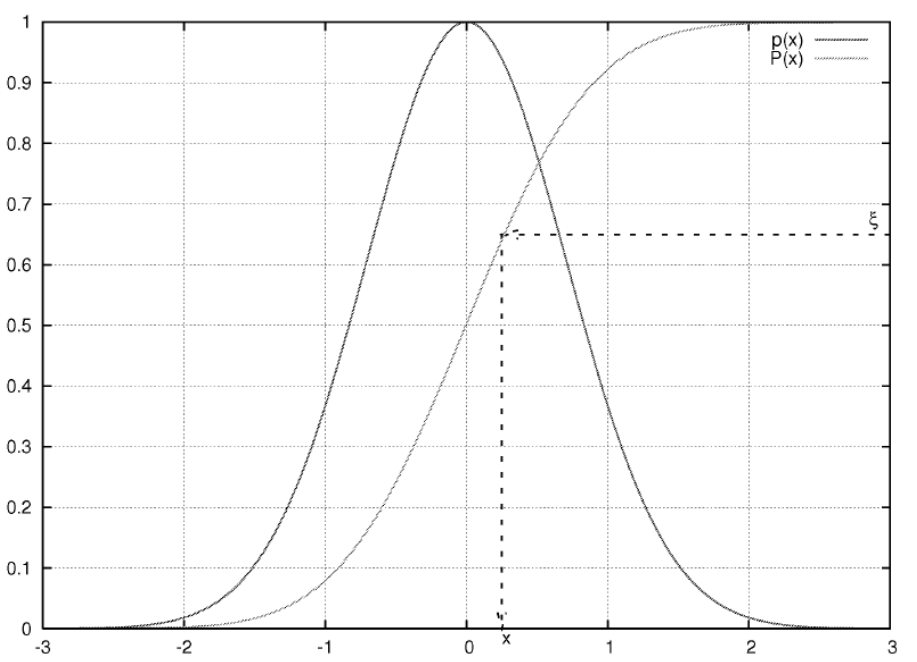
\includegraphics[scale=0.42]{images/trans-inver.PNG}
                \caption{Transformada inversa [2]}
                \label{fig:my_label}
            \end{center}
        \end{figure}
    \end{center}
    
    %fuente: http://nuclear.fis.ucm.es/research/thesis/DEA-jacobo-cal.pdf
\end{itemize}


\begin{comment}
\subsubsection{Generación de números aleatoríos} %pendiente
\noindent Para la generación de números se utilizará el método de la transformada inversa, de esta forma utilizando los datos obtenidos en la aplicación, se puede describir una curva y de esta forma, poder generar números aleatorios, de forma no uniforme, así adaptarse al modelo real en el cual se va a trabajar.
\end{comment}




\subsubsection{Ejemplos} %%%% check 10/24
\noindent Si bien, a la hora de dar una primera definición, ya se ha mencionado un caso para explicar como funciona la simulación de Monte Carlo, a continuación se mostrarán otros ejemplos con el fin de tener mayor claridad de como se llevan a cabo estas simulaciones.

\begin{itemize}
\item Un ejemplo clásico para explicar el método de Monte Carlo es el de dejar caer esferas pequeñas en un área cuadrada, como lo exponen \citeauthor{johansen2007} (\citeyear{johansen2007}), el cual contiene en su centro un recipiente circular de forma tal que el diámetro de la circunferencia sea igual a los lados del rectángulo, como se puede observar en la figura 2.1. Si se dejan caer esferas de manera aleatoria dentro del espacio establecido, se puede tomar una relación entre las esferas que caen dentro del recipiente circular, y aquellas que no. Si bien, en un comienzo esta razón no parezca nada relevante, al repetir el acto de dejar caer esferas en el área, se podrá notar que al alcanzar una cantidad de repeticiones lo suficientemente grande, la razon entre la esferas que caen en el circulo y aquellas que no, se aproxima cada vez más al número $\pi$.
    
    \begin{center}
        \begin{figure}[H]
            \begin{center}
                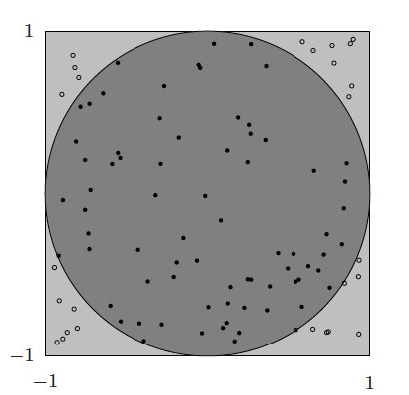
\includegraphics[scale=0.69]{images/montesferas.PNG} % NICE
                \caption{Experimento de esferas [1]}
                \label{fig:my_label}
            \end{center}
        \end{figure}
    \end{center}
    
    \item Otro de los ejemplos clásicos dentro del concepto de Monte Carlo, es el problema de las agujas de Buffon \citep{vargas2020}. Este consiste en dejar caer agujas de manera aleatoria dentro de un espacio determinado y cuyo ángulo de inclinación también es aleatorio. Este ejemplo originalmente recurría a una función trigonométrica para evaluar la inclinación, usando recursivamente el valor de $\pi$ para calcular la función \textit{coseno}, considerandose un error historico, ya que consiste en utilizar el valor de $\pi$ para calcular el mismo.
    
    \begin{center}
        \begin{figure}[H]
            \begin{center}
                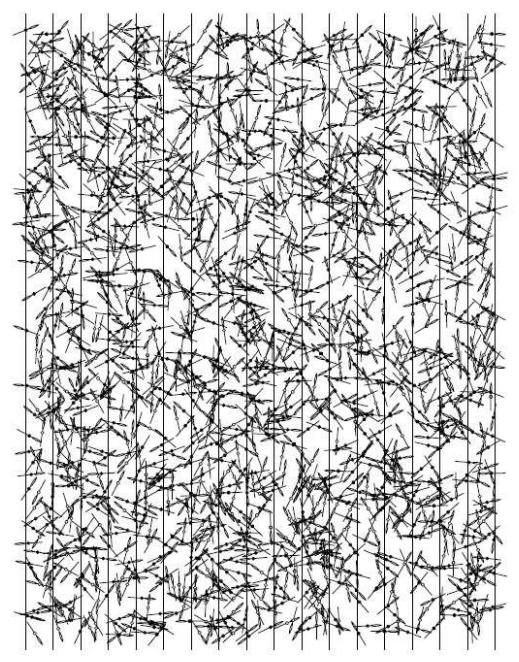
\includegraphics[scale=0.4]{images/agujasbuffon.PNG}
                \caption{Agujas de Buffon [1]}
                \label{fig:my_label}
            \end{center}
        \end{figure}
    \end{center}
    
    Posteriormente, este planteamiento fue corregido, pasando de tomar como factor el grado de inclinación a la generación aleatoria de desplazamientos en los ejes $x$ e $y$, de forma que se lanzaba una enorme cantidad de agujas y se consideraba, por un lado, las agujas que cruzan solo un eje, y por otro, las agujas que cruzan algún eje $x$ y un eje $y$ al mismo tiempo. Teniendo en cuenta que el largo de las agujas es igual que la distancia entre los ejes, se calcula la probabilidad mediante la razón entre las agujas que cruzan una sola linea frente al total de agujas. 
    
    
    
    %ESTUDIO DEL METODO MONTE CARLO EN SIMULACIONES PARA LA ESTIMACION DEL VALOR DE π, J. C. VARGAS & CARLOS ANDRES CRUZ-CARPIO, 2020
    
    \begin{comment}
    \item ejemplo de partículas radioactivas
    %https://www.famaf.unc.edu.ar/~pperez1/manuales/cim/cap6.html  %aaaaaaaaaaaaaaaaaaaaaaaaaaaaa
    \end{comment}
    
\end{itemize}



%%%%%%%%%%%%%%% Teoría de Colas

\subsection{Teoría de Colas} %check 10/24

\noindent El siguiente concepto a explorar es la Teoría de Colas, para la cual, al igual que para la Simulación de Monte Carlo, se comenzará por explicar sus orígenes históricos, continuando con una explicación general de la Teoría, detalles y especificaciones y sus fundamentos teóricos.

\subsubsection{Historia} %%% check 10/24?

\noindent El primer acercamiento a lo que hoy en día se denomina Teoría de Colas fue en el estudio del matemático e ingeniero Agner Erlang sobre la Teoría de Probabilidades en las comunicaciones telefónicas en el año 1909. Erlang trabajó para Copenhagen Telephone Exchange y quería analizar y optimizar sus operaciones. Buscaba determinar cuantos circuitos eran necesarios para proveer un nivel acceptable de servicio telefónico, para que la gente no estuviera "en espera" (o en una cola telefónica) por demasiado tiempo. También tenía curuiosidad sobre averiguar cuantos operadores de teléfonos eran necesarios para procesar cierto volúmne de llamadas. Erlang publicó su primer artículo sobre Teoría de Colas en 1909 donde postuló que se espera que el intercambio telefónico en cierto intervalo de tiempo siga una distribución de Poisson (Erlang, 1909), concluyendo su análisis matemático en su artículo de 1920, "Telephone Waiting Times", el cual sirvió como fundamento de la Teoría de Colas aplicada \citep{queueit2021} \citep{hlynka2017} \citep{mandelbaum2009} \citep{shortle2018}.
\newline \newline
Posteriormente, en 1930 Felix Pollaczek contribuyó con soluciones a problemas de colas, sin embargo ni Erlang ni Pollaczek tenian a disposición la teoría de procesos aleatorios de Markov. Más aún, Pollaczek, sin tener métodos probabilísticos como herramientas, abordaba las problemáticas llevándolas rápidamente a un desarrollo de ecuaciones integrales, lo que en el ámbito de Teoría de Colas generó que sus artículos no tuvieran la llegada que quizas pudieron merecer sus estudios. Hasta ese entonces, solo se habían tratado problemáticas referentes al teletráfico y su comunidad, sin embargo, los estudios de Pollaczek llamaron al atención del matemático ruso Aleksandr Yakovlevich Khinchin, quien continuó resolviendo problemáticas, y es a quien se le atribuye el nexo de las bases establecidas a las probabilidades aplicadas \citep{shortle2018}.
\newline \newline
El primer uso documentado del termino Teoria de Colas (\textit{Queueing Theory}) ocurrió en 1951 en la revista "\textit{Journal of the Royal Statistical Society}", donde David G. Kendall publicó el artículo "\textit{Some Problems in the Theory of Queues}". Si bien existen otros documentos y trabajos respecto al mismo tema, este fue el primer caso en que se usó el termino por el cual se reconocería esta teoría. Además fue Kendall quien propuso la notación A/B/c con la cual se describen las colas comunmente dentro de esta teoría \citep{hlynka2017}.
\newline \newline
Nuevamente, el contexto bélico de la época significó que científicos, sobre todo matemáticos, se unieran a contribuir con problemáticas inusuales, considerando esta vez, enfoques estocásticos. Posterior a la segunda guerra mundial, en 1948, David Kendall, uno de los mencionados matemáticos, tuvo especial curiosidad por el fenómeno de tráfico de comunicaciones y suministros en el marco del bloqueo de Berlin Occidental, y se preguntó si los problemas de evitar la congestión de tráfico se podía estudiar matemáticamente, encontrandose con los estudios de los autores ya mencionados. Si bien sus artículos se catalogaron como expositivos, sirvió para abrir la discusión, llegando a ideas como la de Dennis Lindley, quien propuso abordar la problemática como una relación de recurrencia en base a tiempos de espera en cola, de sevicio y de diferencia entre llegadas a la cola \citep{hlynka2017}.

\subsubsection{Concepto general} %check 10/24

\noindent La teoría de colas corresponde a un conjunto de modelos matemáticos que describen sistemas de líneas de espera específicos. Dado esto, los actores principales que participan en este proceso, son los clientes y los servidores. Se entiende por cliente a los usuarios del servicio por cual se está haciendo la cola, estos usuarios no necesariamente son personas, pueden ser automóviles, ordenes de servicio, etc. Y por servidores, se refiere al prestador del servicio a ser consumido, en el caso que se va a estudiar, por ejemplo, uno de esos servidores podría ser un supermercado.

\subsubsection{Detalles y apreciaciones} %check 10/24

\noindent La figura \ref{figtc} representa una cola de personas utilizando un servicio en particular. Los varios elementos propios que una cola contiene que se explicarán en los siguientes puntos.

    \begin{figure}[H]
        \centering
        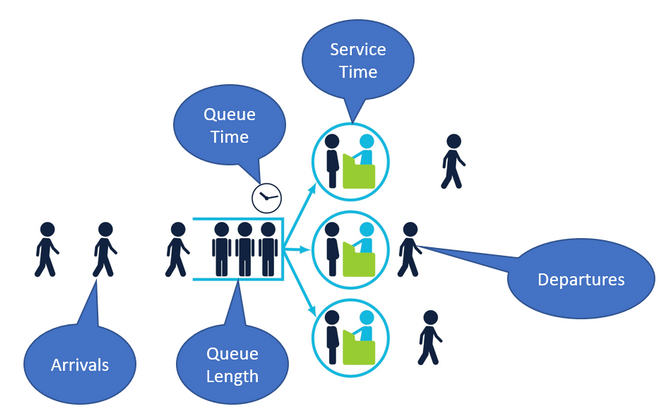
\includegraphics[width=.75\textwidth]{images/Queueing-Example.PNG}
        \caption{Ejemplo de una cola\citep{unknownauthor2021}}
        \label{figtc}
    \end{figure} 
    
\begin{itemize}
    \item \textit{Llegadas}:
    \newline
    En este punto podemos hacer referencias a todo lo que conlleva una llegada a una fila analizada. Podemos destacar los tiempos entre llegada de la cola, las cantidades de usuarios o características de esta, que posea una o más filas, entre otras cosas. Para el caso de estudio sobre el que este documento tiene por contexto, este último punto puede darse existiendo algún tipo de fila presencial o de la misma \'indole.
    
    \item \textit{Capacidad de la cola}:
    \newline
    Este punto hace referencia a la cantidad de usuarios que pueden estar en la cola esperando el servicio. Este punto no siempre es aplicable, ya que las colas pueden ser ilimitadas o no, lo cual puede variar según el modelo del caso de estudio.
    
    \item \textit{Disciplina de la cola}:
    \newline
    Se referiere a cómo se acomodan los usuarios o como salen de la cola, por ejemplo, si corresponde a que el primero en entrar es el primero en salir o el último en entrar es el primero en salir. Si bien esta última no se ve en atenciones a público en general, podemos ver este tipo de colas en procesos computacionales. En casos de atención de servicio a usuarios, se puede dar que existan sistemas de prioridad al momento de entrar al servicio mismo.
    
    \item \textit{Tiempos de espera}:
    \newline
    Corresponde a cuanto tiempo los usuarios tienen que esperar para poder acceder al servicio. Esto puede variar dependiendo del largo de la cola en la que se encuentren o cuantas personas por delante tiene el usuario. Un factor importante con respecto a lo anterior son los tiempos de servicio y la capacidad que pueda brindar. Este apartado en particular es uno de los más importantes a obtener, ya que es uno de los temas de interés a proporcionar mediante el módulo de la aplicación que se quiere realizar.
    
    \item \textit{Tiempos de servicio}:
    \newline
    Puesto que los servicios pueden ser brindados por un solo servidor o servidores múltiples (por ejemplo, en el caso de los supermercados, se pueden tomar como servidores las múltiples cajas al interior de estos), el tiempo de servicio es diferente entre los usuarios, ya que sus tiempos van a ser diferentes. En el caso del supermercado, este tiempo de servicio va a depender de factores como la cantidad de productos que desea llevar o de que tan claro tenga los elementos que desea comprar (por ejemplo, una persona que va a decidir que llevar estando en el supermercado puede que le tome más tiempo que a una persona que sabe de antemano qué va a llevar). Este tiempo de servicio se evalúa como la tasa media de servicio.
    
    \item \textit{Cantidades de servidores}:
    \newline
    Es importante tener en consideración la cantidad de servidores en un estudio para la Teoría de Colas, lo que correponde a un factor de suma importancia, ya que la forma como se comportan los usuarios al estar recibiendo el servicio va a depender de la cantidad de servidores que se tenga. Al haber una mayor cantidad de servidores, los usuarios van a poder repartirse a lo largo de estos, haciendo que las salidas sean más rápidas en comparación a uno de menor cantidad de servidores.\\

    \begin{figure}[H]
        \centering
        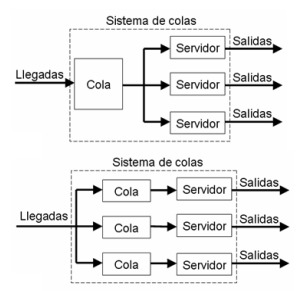
\includegraphics[width=.44\textwidth]{images/colasyservidores.jpeg}
        \caption{Tipos de sistemas de colas [n]} %https://mail.google.com/mail/u/1/#search/mladen.nadinic.c%40usach.cl/FMfcgzGkZGjrxKqMKhgDqtwdLGSCMSNz?projector=1&messagePartId=0.2
        \label{figtc2}
    \end{figure}
    
    Las entradas a los servidores pueden darse de diferentes formas, como se ve en la figura \ref{figtc2}. Cada servidor puede tener colas independientes, o una cola general que se separa para cada servidor. En el caso de estudio que se presenta en esta investigación, y espececíficamente en el caso de las filas externas de los supermercados, se puede apreciar que sea una cola única al exterior, siendo el servicio el supermercado en si, pero al interior del supermercado, podemos ver otro tipo de colas para otros tipos de servidores, ya que existen multiples cajas, siendo un servidor cada caja para poder realizar el pago, lo que también ilustra la figura mencionada.
    
    \item \textit{Salidas}:
    \newline
    La salida, corresponde a las finalización de todo el procedimiento para el usuario, ocurrida una vez que el servicio se ha realizado. Por ejemplo, ya haber concluído el pago en el supermercado y salir de este.
\end{itemize}

\subsubsection{Fundamentos} % check 10/24

\noindent Se utilizará la notación de Kendall para describir el tipo de sistema que se tiene, el cual corresponde a

\begin{center}
A/B/c/N/K
\end{center}

\noindent Correspondiendo a
\begin{itemize}
    \item A: Representa la distribución del tiempo entre llegadas.
    \item B: Representa la distribución del tiempo de servicio.
    \item c: Representa a la cantidad de servicios paralelos.
    \item N: Representa la capacidad del sistema.
    \item K: Representa el tamaño de la población que utiliza el servicio.
\end{itemize}
Se debe tener en cuenta que N y K pueden ser ignorados, en el caso de que estos sean infinitos, quedando los tres primeros elementos. \citep{kendall}

\begin{itemize}
    \item \textit{Ley de Little}:
    \newline
    \noindent Se tiene que la Ley de Little corresponde a
    \begin{equation}
        L=\lambda w\label{eqll}
    \end{equation}
    la cual afirma que el tiempo promedio de clientes en el sistema de una cola, $L$, es igual a la velocidad a la que los clientes llegan y entran al sistema $\lambda$, multiplicado por el promedio tiempo de estancia de un cliente, $w$. %citar: http://www.columbia.edu/~ks20/stochastic-I/stochastic-I-LL.pdf
    \newline\newline
    Profundizando en la Ley de Little, viendo la figura \ref{figll}, que corresponde a una posible realización de un sistema de cola particular, se puede hacer un argumento heur\'isitco sobre la Ley de Little interprentando el \'area bajo la curva de la siguiente imagen

    \begin{figure}[H]
        \centering
        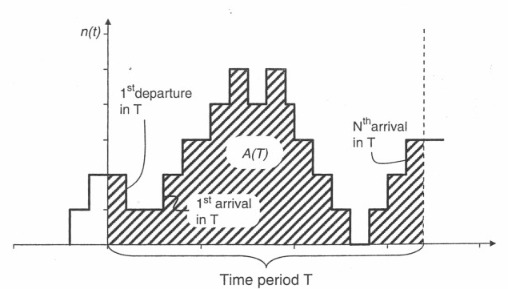
\includegraphics[width=.75\textwidth]{images/littlelaw.jpeg}
        \caption{Cantidad de \'items en el sistema de cola versus tiempo \citep{johndclittle2008}}%http://web.eng.ucsd.edu/~massimo/ECE158A/Handouts_files/Little.pdf
        \label{figll}
    \end{figure} 

    Donde
    \begin{align*}
        n(t) &= \text{el n\'umero de items en la cola en un tiempo $T$}.\\
        T &= \text{Un gran periodo de tiempo}. \\
        A(T) &= \text{el área bajo la curva $n(T)$ en un periodo de tiempo $T$}.\\
        n(T) &= \text{el n\'umero de llegadas en un periodo de tiempo $T$}.
    \end{align*}

    Luego, se define
    \begin{align*}
        \lambda(T) &= \frac{N(T)}{T} = \text{Ritmo de llegada durante un periodo de tiempo $T$}.\\
        K(T) &= \frac{A(T)}{T} = \text{Largo de la cola promedio durante un periodo de tiempo $T$}.\\
        W(T) &= \frac{A(T)}{N(T)} = \text{Tiempo de espera promedio en el sistema por llegada durante $T$}.
    \end{align*}
    Manipulando estas ecuaciones se obtiene,
    \begin{align*}
        L(T) = \lambda(T)W(T)
    \end{align*}
    \begin{adjustwidth}{1.27cm}{}
        Bajo supuestos matemáticos apropiados sobre la estacionariedad del proceso estocástico, los efectos en el inicio y el fin de $T$, se vuelven despreciables comparado con el área bajo la curva principal. Por esto, mientras $T$ crece, estas variaciones estocásticas en $L(T)$, $\lambda(T)$ y $W(T)$ se vuelven más pequeñas y porcentajes más pequeños de sus valores eventuales para que $L(T)$, $\lambda(T)$ y $W(T)$ cada uno por si solo, vayan a un límite mientras $T$ se acerca al infinito. Entoces, llevando estas ideas a ecuaciones matemáticas, se tiene que %http://web.eng.ucsd.edu/~massimo/ECE158A/Handouts_files/Little.pdf
        \begin{align*}
            \lim_{T\to\infty}L(T)&=L;\\
            \lim_{T\to\infty}\lambda(T)&=\lambda;\\
            \lim_{T\to\infty}W(T)&=w,
        \end{align*}
        LLegando con esto, a la ecuación que se postuló en \ref{eqll}.
    \end{adjustwidth}
\end{itemize}


%\subsubsection{Ejemplos}

%%%%%%%%%%%%%%%%%%%%% INTEGRACIÓN DE MONTE CARLO Y TEORÍA DE COLAS

\subsection{Integración de Simulación de Monte Carlo y Teoría de Colas} %check 10/24
\noindent La Teoría de Colas, como se estableció previamente, busca desarrollar un modelo de un sistema físico para simplificar la solución de un problema, por lo que la aplicación de la Teoría de Colas por si sola no entrega soluciones a un problema del mundo real \citep{terrazas2010}. Pero la Teoría de Colas puede utilizarse como herramienta analítica, de modo que se puedan extraer elementos del análisis, para ser observado y optimizado posteriormente con herramientas idóneas para esta tarea.
\newline \newline
Teniendo en cuenta que el enfoque de este trabajo trata un problema cuyos elementos determinantes son de carácter aleatorio, utilizar las simulaciones como método de estudio y análisis que dé paso a una optimización es una etapa natural, más aún tomando particularmente en cuenta las Simulaciones de Monte Carlo, que presentan especial efectividad al tratarse de un sistema que puede llegar a utilizar grandes cantidades de números para establecer el modelo que lo interpreta.
\newline \newline
De este modo, se buscará determinar el modelo detrás de la problemática que se plantea en este documento, identificando los elementos que lo componen, cuáles de estos se pueden determinar fácilmente, y cuáles no se pudieron encontrar y es necesario estimarlos. Para determinar los valores que representan estos elementos no encontrados se utilizará Simulación de Monte Carlo, buscando obtener datos factibles en la vida real, con los cuales se pueda analizar el modelo por completo, obteniendo resultados que sirvan para mejorar el sistema descrito a través del modelo.
\newline \newline
La utilización de simulaciones de Monte Carlo dentro de modelos descritos a traves de Teoría de Colas no es una idea reciente. Diversos estudios y análisis en distintas áreas se han realizado utilizando ambos conceptos para analizar un problema u optimizar un sistema. Para entender los usos que se les han dado a estos conceptos aplicados en conjunto y los resultados que se pueden obtener, se realizará, en los parrafos a continuación, una vista de sólo algunos de los estudios que se han realizado dentro de este contexto, como los dos estudios sobre intoxicación realizados por Guang Wu en 1998, uno sobre intoxicación por inhalación y otro por ingesta de etanol, el estudio de servicios de atención mediante tickets de Chao Yin y el análisis de colas realizado por Yibing Wang, Jingqiu Guo, Avishai (Avi) Ceder, Graham Currie, Wei Don y Hao Yuan sobre servicios de transporte público.

\subsubsection{Ejemplo 1: Teória de Colas y simulación de Monte Carlo en estudios biologícos}

\noindent En 1998, Wu realizó dos trabajos donde incorporaba la Teoría de Colas y Monte Carlo, y estudia, por un lado en la ingesta de etanol (mediante consumo de cerveza) \citep{wu1998eth}, y por otro lado la intoxicación por inhalación (a traves del acto de fumar cigarrillos) \citep{wu1998inh}. Para ambos casos el autor realiza una analogía con Teoría de Colas para modelar el sistema de ingesta y la eliminación de las toxinas del cuerpo. Se utiliza Monte Carlo para simular, en el caso de ingesta de etanol, la cantidad de efectos adversos en función de cantidades de botellas de cerveza y el tiempo necesario para eliminarlos del cuerpo, y para la intoxicación por inhalación, se utiliza Monte Carlo para estimar la cantidad de cigarros acumulados en el sistema respiratorio, y el tiempo necesario para remover estos cigarrillos del cuerpo.
\newline \newline
Hay que tener en cuenta que el autor de ambos estudios da a entender que la analogía entre la función de determinados sistemas biologícos y la Teoría de Colas puede no ser lo suficientemente adecuada en algunos casos. Los resultados de los estudios, si bien correctos e interesantes de estudiar, no son muy factibles en mundo real, y pudiendo realizar cambios al modelo establecido para el sistema de colas, a modo de mejorar el mismo y hacerlo más cercano a un caso real. Por otro lado, puede que los resultados obtenidos puedan parecer contraproducentes, lo que lleva a realizar un mejor estudio y entendimiento del fenómeno (ya que muchos estudios con resultados contraproducentes, como indica el autor, en realidad se deben a que el suceso estudiado no ha sido comprendido del todo).

\subsubsection{Ejemplo 2: Teória de Colas y simulación de Monte Carlo en el servicio de atención mediante tickets}

\noindent En \citeyear{yin2010}, \citeauthor{yin2010} presentó su estudio sobre la simulación de sistemas de servicio de antención mediante tickets basado en el método de Monte Carlo. Este estudio muestra de manera clara el uso de Monte Carlo dentro de los factores que conforman la Teoría de Colas, llevando los elementos del mundo real al modelo que describe el suceso. El estudio pone énfasis en la interacción entre el tiempo promedio de espera de los clientes y el número de ventanillas (servidores) disponibles en momentos establecidos.
\newline \newline
Como resultado, se obtuvo que la cantidad de ventanillas se debe aumentar en una unidad, hasta alcanzar el número máximo de ventanillas, cuando el tiempo promedio de espera de los clientes excede el límite establecido previamente a la hora de realizar la simulación, junto con la cantidad de ventanillas máxima. Este caso, a diferencia de los estudiados por Wu, dan un resultado completamente intuitivo, considerando las limitancias que tiene el sistema en el mundo real, pero tomando ciertos factores del mundo real y considerandolos de manera eficaz dentro del modelo y posterior simulación, obteniendo un resultado que propicia la optimización del sistema.

\subsubsection{Ejemplo 3: Teória de Colas y simulación de Monte Carlo en servicios de transporte público}

\noindent Finalmente, el estudio realizado por \citep{wang2014} trata simulaciones de Monte Carlo a gran escala sobre colas en servicios de transporte público. Dicho documento pone especial énfasis en los comporamientos adversos de los usuarios o clientes de los servicios que ocurren a menudo en la vida real, como lo son usuarios que no respetan las filas o, por impaciencia, deciden salirse de una. Tambien cabe recalcar las variaciones que existen en este trato de la Teoría de Colas, ya que se tienen en cuenta fenómenos que ocurren en el mundo real y que comunmente se ven obviados en la teoría clásica (citar). Conceptos como lotes de arribo, donde los usuarios o clientes llegan a una cola en grupos, y servicio a granel, donde los usuarios o clientes son atendidos de forma grupal, son algunos conceptos que son importantes de distinguir de acuerdo al contexto del suceso que se estudia con la Teoría de Colas. 
\newline \newline
Como resultado, se destaca principalmente el efecto que tienen los comportamientos adversos en la teoría y resultados matemáticos, presentando un modelo analítico basado en lo que los autores denominan, procesos compuestos de Poisson, y la emulación de dichos procesos en las simulaciones de Monte Carlo.

\subsubsection{Conclusiones.}
 \noindent Habiendo mencionado algunos ejemplos de aplicaciones de la Teoría de Colas llevadas a cabo junto con simulaciones de Monte Carlo, podemos sacar algunas conclusiones. En primer lugar, lo variadas que pueden ser las temáticas donde se pueden llevar a cabo este tipo de estudios, con sucesos que a simple vista se pueden visualizar como colas y otros para los cuales es necesario abstraerce del tema principal para encotrar un acercamiento factible. Segundo, pueden existir tantas variaciones a la teoría o al uso de las herramientas, como casos de estudio, donde pequeños cambios o variaciones terminan siendo fundamentales a la hora de construir el modelo y posterior simulación. Tercero y para finalizar, es importante destacar lo vital que es desarrollar y analizar la construcción de los modelos de colas y de simulación, enfocados en el caso de estudio que las convoca, teniendo un conocimiento lo suficientemen comprensivo sobre el tema para poder determinar factores o limitaciones que pueden ser vitales a la hora de obtener resultados y compararlos con los sucesos en la vida real.
\begin{comment}
\newline \newline
Ejemplo 4:
https://www-sciencedirect-com.ezproxy.usach.cl/science/article/pii/S0191261514000307
\end{comment}

%%%%%%%%%%%%%%%%%%%%% Observaciones y alcances de la Teoría de Colas y simulación de Monte Carlo

% \subsection{Observaciones y alcances de la Teoría de Colas y simulación de Monte Carlo en el mundo real}

%A continuación blabla

%%%%%%%%%%%%%%%%%%%%% "Estado del arte"
\subsection{Estudios y aplicaciones afines} %check 10/24
\noindent Dentro de esta sección se encuentran algunos ejemplos de apliaciones de Simulaciones de Monte Carlo y/o Teoría de Colas, pero a diferencia de la sección anterior, en este punto se ven desde el punto de vista del mundo real. También es relevante mencionar el uso de tecnologías móviles, lo cual es parte importante del enfoque del desarrollo dentro de este documento.
\newline \newline
\noindent Cabe destacar el estudio realizado por Mr. Amos Langat, en el 2016, donde se busca la forma predecir volumenes de pacientes en las colas utilizando el método de Monte Carlo. Este estudio fue realizado en Kenia, y dentro de los objetivos que se tienen en esta publicación cabe destacar, con la utilización de esta predicción, reducir los costos de operación en los hospitales. Si bien este estudio no utiliza Teoría de Colas, el proposito final es bastante similar. De la misma forma se puede apreciar que se basa en la utilización de información previa, que en este estudio en particular se obtiene de las planillas de datos del hospital. Para el proyecto que se busca desarolla a lo largo de este documente se plantea, también, utilizar información previa para realizar las simulaciones de Monte Carlo, pero en este caso correponderá a los avisos históricos realizado por los usuarios de la aplicación sobre la cual se realizará el módulo.
\newline \newline
Dentro de la busqueda realizada, se encontraron varias aplicaciones que son interesantes de analizar, por ejemplo la aplicación \textit{Operativa: Queuing Theory}, la cual es una calculadora para Investigación Operativa o Investigación de Operaciones con todos los modelos de Teoría de Colas. %citar:https://alvarez.tech/projects/operativa/
Dentro de las cosas interesantes de este proyecto, si bien no se trata de hacer colas, esta el utilizar uno de los grandes pilares de este proyecto, que es la Teoría de Colas, y más aún, aplicandola sobre tecnologías móviles. Otro punto bastante interesante es que esta aplicación es de código abierto. %(dar alguna justificacion aqui o borrar lo de codigo abierto)
 \newline \newline
Otra aplicación interesante a tener en cuenta es \textit{MobiQueue}. Si bien esta aplicación esta orientada para facilitar a las empresas el servicio al público, de modo que los clientes puedan tomar un número mediante sus celulares y así no tener que hacer filas físicas, la razón de porque esta aplicación es relevante para el estudio es que entrega información de interés tanto a los clientes como a las empresas que contratan este servicio. Por ejemplo, se puede configurar para que lleguen notificaciones vía correo electrónico o mensajes de texto a los clientes sobre el tiempo de espera promedio, utilizando inteligencia artificial. También mediante un tablero entrega información en tiempo real a la empresa utilizando Inteligencia Empresarial (Bussiness intelligence), y finalmente, se pueden extraer reportes de forma periódica. Si bien las aplicaciones se utilizan en ámbitos completamente diferentes, se puede ver que ambas aplicaciones entregan información en base a las filas, por ejemplo, tiempos de espera aproximado e información en tiempo real. %citar: https://mobiqueueapp.com/en
\newline \newline
Finalmente, otras aplicaciones que no hay que dejra de tomar en cuanta en este proyecto son \textit{Waze} y \textit{Moovit}, ya que la lógica inicial es similar. Estas aplicaciónes tienen partes en común aunque sean para fines completamante diferentes. Una de estas partes en común consiste en que los usuarios puedan interactuar con el mapa utilizando su GPS, tambien estos pueden realizar avisos sobre ciertas condiciones provistas por la aplicación. La diferencia consiste en que las aplicaciones señaladas se basan en el desplazamiento de los usuarios por la ciudad, mientras que la aplicación propuesta y sobre la cual se realizará el módulo se basa en avisos sobre las filas de los supermercados. 
 
% EN DUDA: Otra herramienta móvil que se debe tener en cuenta es \textit{E-Queue Mobile Application}
 

%%%%%%%%%%%%%%%%%%%%%%%%%%%%%%%%%%%%%% MARCO METODOLÓGICO

\section{Segunda parte: Marco Metodológico}
\label{sec:segunda}

\subsection{Problemática}
\subsubsection{Descricpción de la problemática}
\subsubsection{Propuesta}

\subsection{Utilización de Monte Carlo dentro de Teoría de Colas}

\subsection{Metodologías de desarrollo}
\subsubsection{Scrum}

%Scrum Un método ágil para sus proyectos (2ª edición)
%Biblioteca ENI: https://www-eni-training-com.ezproxy.usach.cl/portal/client/mediabook/home

\subsubsection{OMT++}

\subsection{Herramientas de desarrollo a utilizar}

El desarrollo de este módulo se va a separar en dos partes, backend y frontend, para esto en se va a crear una API, que la aplicación para android va a consumir, ya sea para ver o publicar información sobre los establecimientos, la parte lógica y donde se impolementará el módulo será en la api.

\subsubsection{Backend}
Para el desarrollo del backend, se va a realizar una API, la cual va a ser desarrollada en el framework
\textit{Ruby on Rails} en su versión 6.1.4. Utilizando el lenguaje de programación Ruby
\newline\newline
La utilización de este framework se va a dividir en las siguientes partes

\begin{itemize}
    \item Modelos
    \item Controladores
    \item Trabajos
    \item Casos de uso (?)
    \item Mailer (?)
\end{itemize}


\subsubsection{Frontend}
Para hacer la aplicación en Android se utilizará el entorno de desarrollo de Android Studio, utilizando el lenguaje \textit{Kotlin} en su versión 4.1.1
\newline\newline
La utilización de este ambiente de desarrollo se va a dividir en las siguientes partes

\begin{itemize}
    \item Componentes
    \item Servicios 
    \item ....
\end{itemize}

\subsection{Casos de uso}
\noindent A continuación, se presentan las tablas que desciben los casos de uso que conforman la aplicación que se toma de base para la implementación del módulo propuesto(, asi como el/los casos de uso que contempla el mismo módulo).

\begin{table}[H]
    \centering
    \caption{Especificación del caso de uso ``Chequear establecimiento"}
    \begin{tabularx}{\textwidth}{|X|X|}
        \hline
        \multicolumn{2}{|l|}{\textbf{Caso de uso N°1:} Chequear establecimiento.}\\\hline
        \multicolumn{2}{|l|}{\textbf{Resumen:} Permite al usuario acceder a la información de los establecimientos en el mapa.}\\\hline
        \multicolumn{2}{|l|}{\textbf{Frecuencia:} Ilimitada.}\\\hline
        \multicolumn{2}{|l|}{\textbf{Actores:} Usuario.}\\\hline
        \multicolumn{2}{|l|}{\textbf{Precondiciones:}}\\
        \multicolumn{2}{|l|}{\begin{minipage}[t]{0.8\textwidth}
        \begin{itemize}
            \item Sesión iniciada en la aplicación.
            %\item GPS activado.
            %\item Acceso a internet.
        \end{itemize}
        \end{minipage}}\\
        \multicolumn{2}{|l|}{}\\\hline
        \multicolumn{2}{|c|}{\textbf{Descripci\'on Flujo Normal (escenario exitoso)}}\\\hline
        \textbf{Responsabilidad del actor:} & \textbf{Responsabilidad del sistema:}\\ \hline
        &1. Mostrar el mapa destacando los establecimientos.\\
        &2. Habilitar opción de seleccionar establecimientos.\\
        3. Seleccionar establecimiento.&\\
        &4. Mostrar información del establecimiento.\\
        &5. Fin caso de uso.\\\hline
        \multicolumn{2}{|l|}{\textbf{Poscondiciones}:}\\
        \multicolumn{2}{|l|}{\begin{minipage}[t]{0,4\textwidth}
        \begin{itemize}
            \item Establecimiento Chequeado.
        \end{itemize}
        \end{minipage}}\\
        \multicolumn{2}{|l|}{}\\\hline        
    \end{tabularx}
    \label{usecase1}
\end{table}

\begin{table}[H]
    \centering
    \caption{Especificaci\'on del caso de uso ``Publicar aviso"}
    \begin{tabularx}{\textwidth}{|X|X|}
        \hline
        \multicolumn{2}{|l|}{\textbf{Caso de uso N°2:} Publicar aviso.}\\\hline
        \multicolumn{2}{|l|}{\textbf{Resumen:} Permite al usuario publicar información de los establecimiento cercanos.}\\\hline
        \multicolumn{2}{|l|}{\textbf{Frecuencia:} Ilimitada.}\\\hline
        \multicolumn{2}{|l|}{\textbf{Actores:} Usuario.}\\\hline
        \multicolumn{2}{|l|}{\textbf{Precondiciones:}}\\
	    \multicolumn{2}{|l|}{\begin{minipage}[t]{0,8\textwidth}
        \begin{itemize}
            \item Caso n°1.
            %\item Usuario a un máximo de 100 metros de distancia del supermercado.
        \end{itemize}
        \end{minipage}}\\
        \multicolumn{2}{|l|}{}\\\hline
        \multicolumn{2}{|c|}{\textbf{Descripci\'on Flujo Normal (escenario exitoso)}}\\\hline
        \textbf{Responsabilidad del actor:} & \textbf{Responsabilidad del sistema:}\\ \hline
        &1. Habilitar opción de publicar aviso de fila.\\
        &2. Habilitar opción de publicar aviso de\\
        &desabastecimiento.\\
        3. Seleccionar publicar aviso.&\\
        &4. Se deriva al caso de uso correspondiente (2.1 o 2.2).\\\hline
        \multicolumn{2}{|l|}{\textbf{Poscondiciones}:}\\
        \multicolumn{2}{|l|}{\begin{minipage}[t]{0,8\textwidth}
        \begin{itemize}
            \item Aviso publicado.
        \end{itemize}
        \end{minipage}}\\
        \multicolumn{2}{|l|}{}\\\hline  
    \end{tabularx}
    \label{usecase2}
\end{table}

\begin{table}[H]
    \centering
    \caption{Especificaci\'on del caso de uso ``Publicar aviso de fila"}
    \begin{tabularx}{\textwidth}{|X|X|}
        \hline
        \multicolumn{2}{|l|}{\textbf{Caso de uso N°3:} Publicar aviso de fila.}\\\hline
        \multicolumn{2}{|l|}{\textbf{Resumen:} Permite al usuario publicar información de las filas del establecimiento.}\\\hline
        \multicolumn{2}{|l|}{\textbf{Frecuencia:} Ilimitada.}\\\hline
        \multicolumn{2}{|l|}{\textbf{Actores:} Usuario}\\\hline
        \multicolumn{2}{|l|}{\textbf{Precondiciones:}}\\
        \multicolumn{2}{|l|}{\begin{minipage}[t]{0,8\textwidth}
        \begin{itemize}
            \item Caso n°2.
            %\item Usuario a un máximo de 100 metros de distancia del supermercado.
        \end{itemize}
        \end{minipage}}\\
        \multicolumn{2}{|l|}{}\\\hline  
        \multicolumn{2}{|c|}{\textbf{Descripci\'on Flujo Normal (escenario exitoso)}}\\\hline
        \textbf{Responsabilidad del actor:} & \textbf{Responsabilidad del sistema:}\\ \hline
        &1. Habilitar opciones de rango de cantidad de personas.\\
        2. Seleccionar rango.&\\
        &3. Mostrar mensaje de confirmación.\\
        &4. Fin caso de uso.\\\hline
        \multicolumn{2}{|l|}{\textbf{Poscondiciones}:}\\
        \multicolumn{2}{|l|}{\begin{minipage}[t]{0,8\textwidth}
        \begin{itemize}
            \item Aviso de fila publicado.
        \end{itemize}
        \end{minipage}}\\
        \multicolumn{2}{|l|}{}\\\hline  
    \end{tabularx}
    \label{usecase3}
\end{table}

\begin{table}[H]
    \centering
    \caption{Especificaci\'on del caso de uso ``Marcar establecimiento como \textit{favorito}"}
    \begin{tabularx}{\textwidth}{|X|X|}
        \hline
        \multicolumn{2}{|l|}{\textbf{Caso de uso N°4:} Marcar establecimiento como \textit{favorito}.}\\\hline
        \multicolumn{2}{|l|}{\textbf{Resumen:} Permite a los usuarios marcar establecimiento como \textit{favorito}}\\\hline
        \multicolumn{2}{|l|}{\textbf{Frecuencia:} Ilimitada.}\\\hline
        \multicolumn{2}{|l|}{\textbf{Actores:} Usuario.}\\\hline
        \multicolumn{2}{|l|}{\textbf{Precondiciones:}}\\
        \multicolumn{2}{|l|}{\begin{minipage}[t]{0.8\textwidth}
        \begin{itemize}
            \item Caso N°1
        \end{itemize}
        \end{minipage}}\\
        \multicolumn{2}{|l|}{}\\\hline
        \multicolumn{2}{|c|}{\textbf{Descripci\'on Flujo Normal (escenario exitoso)}}\\\hline
        \textbf{Responsabilidad del aductor:} & \textbf{Responsabilidad del sistema:}\\ \hline
        &1. Habilitar opción de marcar establecimiento como \textit{favorito}.\\
        2. Seleccionar establecimiento como \textit{favorito}.&\\
        &3. Fin caso de uso.\\\hline
        \multicolumn{2}{|l|}{\textbf{Poscondiciones}:}\\
        \multicolumn{2}{|l|}{\begin{minipage}[t]{0,4\textwidth}
        \begin{itemize}
            \item Establecimento favorito.
        \end{itemize}
        \end{minipage}}\\
        \multicolumn{2}{|l|}{}\\\hline        
    \end{tabularx}
    \label{usecase4}
\end{table}

\begin{table}[H]
    \centering
    \caption{Especificaci\'on del caso de uso ``Desmarcar establecimiento como \textit{favorito}"}
    \begin{tabularx}{\textwidth}{|X|X|}
        \hline
        \multicolumn{2}{|l|}{\textbf{Caso de uso N°5:} Desmarcar establecimiento como favorito}\\\hline
        \multicolumn{2}{|l|}{\textbf{Resumen:} Permite a los usuarios desmarcar un establecimiento como favorito}\\\hline
        \multicolumn{2}{|l|}{\textbf{Frecuencia:} Ilimitada.}\\\hline
        \multicolumn{2}{|l|}{\textbf{Actores:} Usuario.}\\\hline
        \multicolumn{2}{|l|}{\textbf{Precondiciones:}}\\
        \multicolumn{2}{|l|}{\begin{minipage}[t]{0.8\textwidth}
        \begin{itemize}
            \item Caso N°1
            \item Caso N°4
        \end{itemize}
        \end{minipage}}\\
        \multicolumn{2}{|l|}{}\\\hline
        \multicolumn{2}{|c|}{\textbf{Descripci\'on Flujo Normal (escenario exitoso)}}\\\hline
        \textbf{Responsabilidad del aductor:} & \textbf{Responsabilidad del sistema:}\\ \hline
        &1. Habilitar opción de desmarcar establecimiento como favorito.\\
        2. Deseleccionar establecimiento como favorito.&\\
        &3. Fin caso de uso.\\\hline
        \multicolumn{2}{|l|}{\textbf{Poscondiciones}:}\\
        \multicolumn{2}{|l|}{\begin{minipage}[t]{0,4\textwidth}
        \begin{itemize}
            \item Establecimiento no favorito.
        \end{itemize}
        \end{minipage}}\\
        \multicolumn{2}{|l|}{}\\\hline        
    \end{tabularx}
    \label{usecase5}
\end{table}

\begin{table}[H]
    \centering
    \caption{Especificaci\'on del caso de uso ``A"}
    \begin{tabularx}{\textwidth}{|X|X|}
        \hline
        \multicolumn{2}{|l|}{\textbf{Caso de uso N°X:} }\\\hline
        \multicolumn{2}{|l|}{\textbf{Resumen:} }\\\hline
        \multicolumn{2}{|l|}{\textbf{Frecuencia:} }\\\hline
        \multicolumn{2}{|l|}{\textbf{Actores:} }\\\hline
        \multicolumn{2}{|l|}{\textbf{Precondiciones:}}\\
        \multicolumn{2}{|l|}{\begin{minipage}[t]{0.8\textwidth}
        \begin{itemize}
            \item Caso N°X
        \end{itemize}
        \end{minipage}}\\
        \multicolumn{2}{|l|}{}\\\hline
        \multicolumn{2}{|c|}{\textbf{Descripci\'on Flujo Normal (escenario exitoso)}}\\\hline
        \textbf{Responsabilidad del aductor:} & \textbf{Responsabilidad del sistema:}\\ \hline
        &1. Habilitar opción de desmarcar establecimiento como favorito.\\
        2. Deseleccionar establecimiento como favorito.&\\
        &3. Fin caso de uso.\\\hline
        \multicolumn{2}{|l|}{\textbf{Poscondiciones}:}\\
        \multicolumn{2}{|l|}{\begin{minipage}[t]{0,4\textwidth}
        \begin{itemize}
            \item Establecimiento no favorito.
        \end{itemize}
        \end{minipage}}\\
        \multicolumn{2}{|l|}{}\\\hline        
    \end{tabularx}
    \label{usecase5}
\end{table}

\subsection{Modelo de la Base de Datos}



% \section{Tercera parte}
% \label{sec:tercera}
% Actualmente el Departamento cuenta con 14 académicos jornada completa y tres investigadores asociados, de los cuales un 95\% tiene grado de Doctor. Se están ejecutando más de una decena de proyectos de investigación, en diferentes áreas. Además la productividad científica se expresa en más de 25 publicaciones en revistas indexadas en los últimos 5 años.

% \begin{algorithm}[!ht]
% 	\caption{Algoritmo de ejemplo.}
% 	\label{alg:ejemplo}
% 	\begin{algorithmic}[1]
% 	\REQUIRE Entrada de ejemplo.
% 	\ENSURE Salida de ejemplo.	
	
% 	\IF {esto est\'a bien}
% 		\STATE hacer algo
% 	\ELSE
% 		\STATE hacer otra cosa
% 	\ENDIF
	
% 	\RETURN Retornar ejemplo
	
% 	\end{algorithmic}
% \end{algorithm}

% \section{Cuarta parte}
% \label{sec:cuarta}
% Desde el año 1972, con la creación de la carrera de Ingeniería de Ejecución en Computación e Informática, la UdeSantiago comenzó un proceso  de formación de un cuerpo académico de excelencia, que se ha ido involucrando en proyectos cada vez más ambiciosos, en zonas de frontera tecnológica en diversas áreas aplicativas de la informática la Ecuación \ref{eq:ejemplo}.

% \begin{equation}
% 	A = B + C
% \label{eq:ejemplo}
% \end{equation}

% \chapter{Conclusiones}
% \label{cap:conclusiones}
% La carrera de Ingeniería de Ejecución en Computación e Informática antecede la aparición del Departamento de Ingeniería Informática por diez años. Ella comenzó a dictarse en 1972 bajo la responsabilidad del Centro de Computación de la UTE (CECUTE) y se regularizó su creación por medio del Decreto 944 de 1975, el que establece su dependencia de la Facultad de Ingeniería. Los primeros Ingenieros de Ejecución en Computación e Informática comenzaron a titularse en el año 1976 \citep{delgado2016exposicion}.

{\setstretch{1.0}						% Interlineado en las páginas finales
% ### Optativo: Glosario ###
\clearpage
\addcontentsline{toc}{chapter}{Glosario}
\glosario{

% CMS: Un Sistema de gestión de contenidos (Content Management System en inglés, abreviado CMS) es un programa que permite crear una estructura de soporte (framework) para la creación y administración de contenidos, principalmente en páginas web, por parte de los participantes. Consiste en una interfaz que controla una o varias bases de datos donde se aloja el contenido del sitio. El sistema permite manejar de manera independiente el contenido y el diseño. Así, es posible manejar el contenido y darle en cualquier momento un diseño distinto al sitio sin tener que darle formato al contenido de nuevo, además de permitir la fácil y controlada publicación en el sitio a varios editores.

% Copyleft: Es una forma de licencia y puede ser usado para modificar el derecho de autor de obras o trabajos, tales como software de computadoras, documentos, música, y obras de arte. Bajo tales licencias pueden protegerse una gran diversidad de obras, tales como programas informáticos, arte, cultura y ciencia, es decir prácticamente casi cualquier tipo de producción creativa.

% Creative Commons: Es una organización no gubernamental sin ánimo de lucro que desarrolla planes para ayudar a reducir las barreras legales de la creatividad, por medio de nueva legislación y nuevas tecnologías. Fue fundada por Lawrence Lessig, profesor de derecho en la Universidad de Stanford y especialista en ciberderecho, que la presidió hasta marzo de 2008.

% Distribución GNU/Linux: Versión de GNU/Linux que agrupa una serie de programas, que es organizada y mantenida adelante por algún grupo, empresa o institución.

% Drupal: Es un programa de código abierto, con licencia GNU/GPL, escrito en PHP, desarrollado y mantenido por una activa comunidad de usuarios. Destaca por la cálidad de su código y de las páginas generadas, el respeto de los estándares de la web, y un énfasis especial en la usabilidad y consistencia de todo el sistema.

% RSS: Es el acrónimo de Really Simple Syndication, una familia de formatos utilizada para publicar frecuentemente contenidos actualizados, como entradas de blogs o titulares de noticias. Un documento RSS puede contener un resumen de su contenido de un sitio web asociado o su texto completo.

}

% ### Bibliografía de la tesis ###
\clearpage
\addcontentsline{toc}{chapter}{Referencias bibliogr\'aficas} % Comando para agregar el índice a la Tabla de
\bibliographystyle{apa-good}
\bibliography{bibliografia}

% ### Optativo: Anexos de la tesis ###
\clearpage
\anexo
\addcontentsline{toc}{chapter}{Anexos}

% \chapter{Título del anexo ejemplo}
% \label{finales:anexo1}
% El 15 de junio del 2012 la Agencia Acreditadora Colegio de Ingenieros de Chile S.A., otorga la acreditación de la carrera de Ingeniería Civil Informática de la Universidad de Santiago de Chile sede Santiago, en sus jornadas diurna y vespertinas por un plazo de 5 años.
% ### Anexos ###

% ### Optativo: Apéndices de la tesis ###
\clearpage
\apendice
\addcontentsline{toc}{chapter}{Apéndices}

% ### Apéndices ###
% \chapter{Título del apéndice ejemplo}
% \label{finales:apendice1}
 % El 15 de junio del 2012 la Agencia Acreditadora Colegio de Ingenieros de Chile S.A., otorga la acreditación de la carrera de Ingeniería Civil Informática de la Universidad de Santiago de Chile sede Santiago, en sus jornadas diurna y vespertinas por un plazo de 5 años.
} % end \setstretch{1.0}

\end{document}
% end